% UTF-8

% single-chapter commands
\documentclass[../main/thesis.tex]{subfiles}
\onlyinsubfile{\setcounter{chapter}{4}}  % single-chapter command
\begin{document}


\chapter{Implementierung}

\section{Entwicklungsumgebung}

Zur Umsetzung der entwickelten Algorithmen in Software wurde die Plattform Java verwendet.
Die Wahl von Java erfolgte neben der Vertrautheit des Verfassers mit dem zugehörigen \term{framework} aufgrund zu erwartender Effizienzvorteile von kompiliertem Code gegenüber Skriptsprachen wie Perl.
% einer Empfehlung der Geofabrik folgend

Java als imperative Sprache erlaubt es nicht, Algorithmen mit dem gleichen Grad an Abstraktion zu beschreiben wie zuvor in Kapitel~\ref{ch:algorithm-parts} geschehen.
Dort konnten zugunsten einer vereinfachten
% jedoch präzisen, cf. EWD656
Beschreibung praktische Erwägungen wie der Bedarf an Rechenzeit und Speicherplatz teilweise hintenanstehen.
Bei der Implementierung in Java müssen hingegen sorgfältig solche Datenstrukturen gewählt werden, die eine effiziente Ausführung erlauben, und die Algorithmen soweit nötig entsprechend angepasst werden.
Das Ergebnis wird in Abschnitt~\ref{ch:data-structures} beschrieben.

Während der Entwicklung wurde versucht, so viel existierenden Code in Form von \term{frameworks} wiederzuverwenden wie möglich.
Diese Bestrebung verursachte Probleme, wie auch später in Abschnitt~\ref{ch:impl-difficulties} geschildert wird.
Bei der Entwicklung kamen zuletzt die folgenden Plattformen und \term{frameworks} zum Einsatz:

\begin{itemize}[nosep]
	\item Darwin 15.6 / Mac OS X 10.11.6
	\item Java™ Standard Edition JDK 8 Update 152\\ \url{http://www.oracle.com/technetwork/java/javase/downloads/}
	\item Apache Ant 1.10.1 \quad \url{https://ant.apache.org/}
	\item args4j 2.33 \quad \url{http://args4j.kohsuke.org/}
	\item GeoTools 18.0 \quad \url{http://www.geotools.org/}
	\item TestNG 6.8 \quad \url{http://testng.org/}
	% http://web.archive.org/web/20121113133417/http://testng.org/testng-6.8.zip (all other releases appear to be corrupt; I'm probably doing something wrong)
	\item GDAL 2.2.2 \quad \url{http://www.gdal.org/}
\end{itemize}

Ursprünglich wurden ältere Softwareversionen verwendet.
Die nötigen Anpassungen an die hier genannten aktuellen Versionen waren gering, Kompatibilität mit den älteren Versionen ist jedoch gegenwärtig aufgrund von Änderungen in GeoTools nicht mehr vollständig gegeben.
Der Code ist dabei noch immer konform zum Syntax von Java 6. \cf{GJSB05}

Der folgende Abschnitt erläutert einige Überlegungen, die bei der Auswahl der \term{frameworks} relevant waren.



\section{Systemarchitektur}

Für ein gut funktionierendes Gesamtpaket sind vor der Umsetzung von vorgegebenen Algorithmen in ausführbarem Code einige praktische Aspekte zu bedenken.

Zunächst stellt sich die Frage nach der Benutzerschnittstelle der Software.
Die gewählte Plattform Java bietet verschiedene Möglichkeiten, graphische Benutzeroberflächen (GUI) zu gestalten.
Denkbar wäre beispielsweise eine Integration in den weit verbreiteten \osm-Editor JOSM als \term{plug-in.}
Das Entwickeln und Debuggen einer GUI-Anwendung neigt jedoch dazu, zeitaufwändig zu sein.
Ohnehin würde es ein modularer Aufbau der Anwendung erlauben, zu einem späteren Zeitpunkt eine optionale GUI zu ergänzen.
\cf[171]{Muc05}
Aus diesen Gründen soll im Rahmen dieser Arbeit auf eine GUI zugunsten einer einfachen textbasierten Kommandozeilen-Schnittstelle (\term{command-line interface,} CLI) verzichtet werden.
Zum Parsen der CLI-Parameter bieten sich einfache \term{frameworks} wie etwa args4j an.

Zur Verarbeitung beliebiger Geodaten müssen diese aus Datenspeichern eingelesen und wieder ausgegeben werden können.
Um Entwicklungszeit zu sparen, sollte hierfür nach Möglichkeit ein existierendes \term{framework} genutzt werden.
Zur Vermeidung einer zu engen Kopplung der Generalisierung an das gewählte \term{framework} ist es zu vermeiden, die Primitiven des \term{frameworks} intern weiterzubenutzen.
% -> ???
Stattdessen sollten eigene Datenstrukturen genutzt werden, um Modularität zu fördern.
Die dabei entstehenden Kosten in Form von Rechenzeit und Speicherverbrauch sind zu berücksichtigen.

Da die Algorithmen auf der euklidischen Ebene definiert sind (vgl. Abschnitt~\ref{ch:split-algorithm}), bietet es sich an, die Implementierung zunächst auf kartesische Koordinaten zu beschränken und zu verlangen, dass aus der \osm-Datenbank stammende Eingangsdaten nach Länge und Breite vor der Verarbeitung vom Benutzer in einem geeigneten Kartennetzentwurf abgebildet werden.
% Achtung: das passiert im ShapeReader automatisch, wenn die Eingangsdaten eine Abbildung vorgeben! -> Text hier anpassen!
Grundsätzlich wären angesichts der hier durchzuführenden geometrischen Operationen winkeltreue Abbildungen wie etwa ein Mercator-Netz zu bevorzugen.
\cf[20]{Sny87}
Aufgrund der üblicherweise geringen Abstände der Parallelen ist Winkeltreue jedoch kein strenges Kriterium.
% Wiederholung eines ähnlichen Gedanken in 4.3.1

Die in Abschnitt~\ref{ch:split-algorithm} gegebene Definition für \textproc{NaheSegmente} kann leicht mit Hilfe eines R-Baums als räumlicher Index umgesetzt werden.
Die \textproc{Hülle} ist dabei das minimal umgebende Rechteck eines Blatts im R-Baum.
Nachdem die \osm-Eingangsdaten vor der Generalisierung vollständig bekannt und somit statisch sind, bietet sich der Einsatz eines gepackten R-Baums an \cf[255-256]{RSV02}.
Ein solcher Baum wird von der JTS Topology Suite (JTS) angeboten, welche vom \term{framework} GeoTools als Implementierung des Geometriemodells verwendet wird.

GeoTools bietet außerdem Möglichkeiten zur Ein- und Ausgabe (\term{input/output,} I/O) von Geodaten in zahlreichen Formaten.
Zwar wird das native \osm-XML-Format ebensowenig unterstützt wie das neuere Protocol Buffer Binary Format (PBF).
Das verbreitete Format ESRI~Shapefile wird jedoch unterstützt.
Die Geofabrik stellt aktuelle OSM-Auszüge öffentlich als Shapefile bereit.
Alternativ lassen sich Shapefiles leicht mit gängiger Software wie etwa GDAL aus anderen Formaten erzeugen.
GDAL ermöglicht dabei auch den Zuschnitt auf ein abgegrenztes Untersuchungsgebiet, was sich für Testzwecke anbietet.

\onefigure{ht}{
	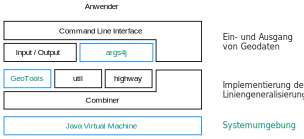
\includegraphics[width=\ScaleIfNeeded]{../chapter5/system-concept}
	\caption{Systemkonzept (schwarz: eigene Entwicklung, blau: benutztes \term{framework})}
	\label{fig:system-concept}
}

Zusammengesetzt ergibt sich aus den besprochenen Aspekten die in Abbildung~\ref{fig:system-concept} dargestellte Architektur:
Dem Anwender steht eine Kommandozeilen-Schnittstelle (CLI) zur Verfügung, die ihrerseits das \term{framework} args4j zum Parsen der Parameter sowie selbst entwickelte Routinen zur Ein- und Ausgabe der Geodaten verwendet.
Die CLI steuert damit die eigentliche Liniengeneralisierung (hier als „Combiner“ bezeichnet), welche ihrerseits neben dem \term{framework} GeoTools noch einige selbst entwickelte Hilfsmodule verwendet, die nicht vom Combiner abhängig sind und deshalb als separates Softwarepaket dargestellt werden (mit „util“ bezeichnet).
Schließlich sitzt zwischen Combiner und CLI ein mit „highway“ bezeichnetes Paket, welches versucht, die Logik des in Abschnitt~\ref{ch:case-selection} ausgewählten Spezialfalls an einem Ort zu bündeln, um die Anpassung auf andere Spezialfälle zu erleichtern.

% Noch mal Modularisierung; java Packages erwähnen/erklären? -> eher nein

Im folgenden Abschnitt wird näher auf die Implementierung der Liniengeneralisierung insbesondere im Combiner eingegangen.



\section{Datenstrukturen}
\label{ch:data-structures}

% - übergeordnete Frage: warum _so_ und nicht anders?

Aus Gründen der Übersichtlichkeit werden in den folgenden Abschnitten nur wesentliche Aspekte und wichtige Entscheidungen behandelt.
Für Detailfragen sei auf die Dokumentation der Programmierschnittstelle verwiesen, welche in englischer Sprache als Teil der Softwareentwicklung im Javadoc-Format angelegt wurde und sowohl im Java-Quellcode als auch im HTML-Format zugänglich ist.



\subsection{Grundlegendes Geometrie-Modell (GeoTools)}

Zur Umsetzung der in Abschnitt~\ref{ch:algorithm-parts} definierten geometrischen Algorithmen werden zunächst Strukturen zur Repräsentation der grundlegenden Datentypen benötigt.
Im Kontext dieses Projekts sind dies:
\begin{enumerate}[nosep]
	\item Punkt (\osm-\term{node})
	\item Segment (Verbindung von zwei Punkten als Teil eines Linienzugs)
	\item Linienzug (\osm-\term{way})
\end{enumerate}

\noindent
Das \term{framework} GeoTools benutzt dazu die JTS Topology Suite, die wie zuvor beschrieben ohnehin wegen des R-Baums für \textproc{NaheSegmente} zum Einsatz kommen soll.
JTS bietet mit der \code{Geometry}-Hierarchie Datenstrukturen nach ISO~19125\hbox{-}1 an, die grundsätzlich auch für die Implementierung der Algorithmen aus Abschnitt~\ref{ch:algorithm-parts} geeignet wären.
% http://atetric.com/atetric/javadoc/com.vividsolutions/jts-core/1.14.0/com/vividsolutions/jts/geom/package-summary.html

Die Algorithmen \textproc{Splitten} und \textproc{Analyse} ordnen den Segmenten allerdings zusätzliche Attribute zu ($wurzel$ bzw. $parallelLinks / parallelRechts$).
Dies unterstützt JTS zwar in Form von \term{user data objects}.
% http://atetric.com/atetric/javadoc/com.vividsolutions/jts-core/1.14.0/com/vividsolutions/jts/geom/Geometry.html#getUserData--
Weil jedoch die Arbeit damit eher umständlich ist, wäre dies nur sinnvoll, wenn die Nutzung der JTS-Datenstrukturen andere Vorteile bietet.

Dies ist jedoch nicht der Fall.
Im Gegenteil passen die JTS-Datenstrukturen nicht gut auf die definierten Algorithmen:
Diese beschränken sich zu einem großen Teil auf Segmente aus exakt zwei Punkten, während JTS von längeren Linienzügen ausgeht.
Die Algorithmen machen sich außerdem zunutze, dass sich Segmente direkt als Vektoren interpretieren lassen (vergleiche Abschnitt~\ref{ch:split-algorithm}).
Routinen zur Vektor-Mathematik bietet JTS zwar grundsätzlich an, jedoch sind wichtige Teile davon nicht spezifiziert.
Beispielhaft sei die Klasse \code{jts.math.Vector2D} genannt, deren Methode \code{angle()} offenbar Winkel berechnet, jedoch in keiner Weise dokumentiert ist.
% http://atetric.com/atetric/javadoc/com.vividsolutions/jts-core/1.14.0/com/vividsolutions/jts/math/Vector2D.html
Die Definition der \textproc{Analyse} auf Parallelität verlangt jedoch einen bestimmten Wertebereich für Winkel von Vektoren.
Obwohl sich die derzeitige Implementierung von \code{angle()} leicht anhand des Quellcodes von JTS ermitteln ließe, ist die Methode nicht zuverlässig verwendbar, weil ohne Dokumentation bereits unklar bleibt, ob die derzeitige Implementierung überhaupt korrekt ist.

Hinzu kommt, dass auch die von JTS angebotenen Operationen zur Manipulation geometrischer Daten -- abgesehen vom räumlichen Index -- hier wenig hilfreich sind.
Ein direktes Verwenden der bereitgestellten JTS-Datenstrukturen erscheint folglich insgesamt betrachtet nicht sinnvoll zu sein.
Stattdessen wurde ein eigenes Datenmodell entwickelt, das im Folgenden beschrieben wird.

JTS bietet die Möglichkeit, das \term{framework} zusammen mit eigenen Datenstrukturen zu benutzten, wenn diese bestimmte Schnittstellen anbieten.
% z. B. CoordinateSequence
% wie in Nr. 8 im "JTS Topology Suite Developer’s Guide" 1.4 beschrieben
Dies käme hier durchaus in Betracht, damit die eigenen Datenstrukturen zukünftig von Dritten unmittelbar mit JTS genutzt werden können.
Beispielsweise könnten so zusammengefasste Linienzüge als Ergebnisse der hier entwickelten Software direkt mit JTS einer Formvereinfachung unterzogen werden.
Weil dies jedoch nicht Bestandteil dieser Arbeit ist und ein Implementieren jener Schnittstellen keinen direkten Nutzen hat, wurde darauf zunächst verzichtet.
Es ließe sich für eine zukünftige Version leicht ergänzen.



\subsection{Grundlegendes Geometrie-Modell (eigene Entwicklung)}

Ein vollständiges Diagramm des entwickelten Datenmodells ist dem Anhang zu entnehmen.
Vereinfacht auf die grundlegenden Geometrie-Datentypen ergibt sich das in Abbildung~\ref{fig:impl-geometry-model} gezeigte Datenmodell.
Die Segmente sind wie in Abschnitt~\ref{ch:split-algorithm} beschrieben zunächst nicht in den Eingangsdaten vorhanden; sie daraus durch \textproc{Segmentierung} herzustellen, ist jedoch nahezu trivial.

%   https://de.wikipedia.org/wiki/Assoziation_(UML)#Aggregation_und_Komposition

\onefigure{ht}{
% [Dataset]1 <>-- 0…n[Line]1 <>-- 1…n[Segment]1…n <>-- 2[Node]
	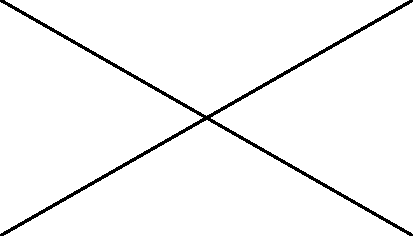
\includegraphics[width=\ScaleIfNeeded]{../image-missing}
	\\\texttt{ [Dataset]<>--[Line]<>--[Segment]<>--[Node]}
	\\\texttt{~~~~~~~~~1~~~0…n~~~1~~~1…n~~~~~1…n~~~2~~~~~}
	\caption{...}
	\label{fig:impl-geometry-model}
}

Die hier gezeigten Datentypen wurden als Interfaces (formale Schnittstellendefinitionen) umgesetzt, um ihre eventuelle Wiederverwendung zu erleichtern. \cf[18]{GHJV95}
Abbildung~\ref{fig:impl-class-structure-splitting} zeigt die bei der Implementierung dieses Datenmodells entstandene Klassenstruktur.

\onefigure{ht}{
% [Klassenstruktur "Splitten"]
	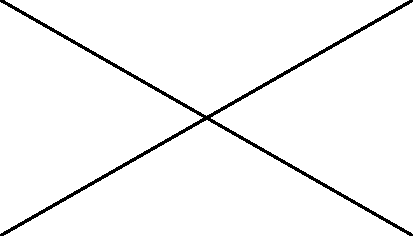
\includegraphics[width=\ScaleIfNeeded]{../image-missing}
	\caption{Klassenstruktur „Splitten“}
	\label{fig:impl-class-structure-splitting}
}

Die Anzahl der jeweils das Interface implementierenden Klassen ist in diesem Projekt klein, so dass es sich anbietet, die jeweiligen Gemeinsamkeiten in abstrakten Klassen
% wie \code{AbstractSegment}
zusammenzufassen, um Redundanzen zu vermeiden.
Diese Klassen gehören daher zu den umfangreicheren im Projekt.
% Herauszustellen ist insbesondere die Klasse \code{AbstractSegment}, welche u.~a. wichtige Algorithmen wie \textproc{Fußpunkt} und \textproc{Analyse} enthält.

Wie in Abschnitt~\ref{ch:split-algorithm} erläutert, existiert derjenige \term{node}, an dem Segmente beim \textproc{Splitten} zerteilt werden, nicht in den Eingangsdaten.
Dementsprechend wird unterschieden zwischen \code{SourceNode} (aus den \osm-Quelldaten kommend) und \code{NonexistentNode} (beim \textproc{Splitten} entstehend).
Beide implementieren jedoch die gemeinsame Schnittstelle für den Typ \code{Node}.
Zu den Gemeinsamkeiten beider Arten von \code{Node}s gehören in erster Linie deren Koordinaten, welche folglich die Klasse \code{AbstractNode} verwaltet und an die beiden konkreten Implementierungen vererbt.

In gleicher Weise fasst \code{AbstractSegment} Gemeinsamkeiten solcher Segmente, die direkt aus den Eingangsdaten stammen (\code{SourceSegment}), und solcher Segmente, die erst durch \textproc{Splitten} eines anderen Segments entstehen (\code{Fragment}), zusammen.
In Abschnitt~\ref{ch:algorithm-parts} wurden solche Segmente zur Vereinfachung einander gleichgestellt.
Für derartige Fälle schlagen Gamma et~al. den Einsatz des Kompositum-Entwurfsmusters vor:
„Use the Composite pattern when [...] you want clients to be able to ignore the difference between compositions of objects and individual objects. Clients will treat all objects in the composite structure uniformly.“ \citex[164]{GHJV95}
Im Kompositum-Muster werden Objekte zu Baumstrukturen aus individuellen Objekten (Blättern) und Komposita von Objekten zusammengefügt.

Im Kontext des Kompositum-Musters ist jedoch die Besonderheit zu berücksichtigen, dass hier einige Blätter aus den Eingangsdaten stammen (\code{SourceSegment}s), andere nicht (\code{Fragment}s).
Gleiches gilt auch für Komposita, so dass sich in einer nur auf Vererbung bestehenden Klassenstruktur sofort eine Wucherung aus größtenteils redundanten Klassen ergäbe.
Für solche Fälle schlagen Gamma et~al. vor, das Brücken-Muster \term{(Bridge pattern)} einzusetzen, mit dem die Redundanz durch Delegation vermieden werden kann. \cf[153]{GHJV95}

\onefigure{ht}{
	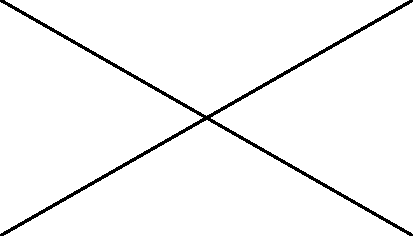
\includegraphics[width=\ScaleIfNeeded]{../image-missing}
	\caption{Composite-Bridge}
	\label{fig:impl-composite-bridge}
}

Eine Kombination aus Kompositum und Brücke wäre zwar möglich, würde jedoch zu einer recht unübersichtlichen Struktur führen.
Gamma et~al. betonen, dass Delegation unweigerlich Komplexität mit sich bringt und nur dann sinnvoll ist, wenn andere Vorteile überwiegen („Delegation is a good design choice only when it simplifies more than it complicates.“ \citex[21]{GHJV95}).
Dies wäre hier offensichtlich nicht der Fall (Abbildung~\ref{fig:impl-composite-bridge}).
Ihre Empfehlung, Delegation möglichst nur in Form von standardisierten Mustern zu verwenden, [\cfibid] scheint hier auch wegen einer weiteren Besonderheit nicht anwendbar zu sein:

Alle Objekte im \code{AbstractSegment}-Kompositum sind veränderbar (\term{mutable}), damit bei der Umwandlung von Blättern (die jeweils ein Segment repräsentieren) in Komposita (die zwei oder mehr Segmente repräsentieren) beim \textproc{Splitten} keine großen Kosten entstehen.
Bloch betont die erheblichen Vorteile von \term{immutability} (\emph{nicht} veränderbarer Objekte), weist aber auch darauf hin, dass bestimmte komplexe Operationen dann sehr teuer werden können („The performance problem is magnified if you perform a multistep operation that generates a new object at every step, eventually discarding all objects except the final result.“ \citex[67]{Blo01}).
Im vorliegenden Kompositum würde \term{immutability} gerade erfordern, dass bei jedem \textproc{Splitten} der Baum neu aufgebaut wird.

Unterschiedliche Klassen für Blätter und Komposita sind deshalb hier gar nicht angebracht; vielmehr bietet es sich \emph{in Anlehnung an} standardisierte Muster an, dass eine gemeinsame Klasse mit einem Attribut \term{children} sich entweder wie ein Blatt oder wie ein Kompositum verhält, je nachdem, ob es \term{children} in Form von Fragmenten gibt oder nicht.

\onefigure{ht}{
	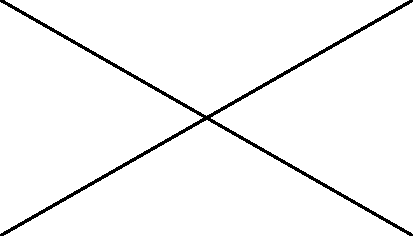
\includegraphics[width=\ScaleIfNeeded]{../image-missing}
	\caption{Composite (IST)}
	\label{fig:impl-class-structure-composite}
}

Aus dieser Erkenntnis ergibt sich eine vergleichsweise einfache Klassenstruktur (Abbildung~\ref{fig:impl-class-structure-composite}):
\code{AbstractSegment} implementiert die Gemeinsamkeiten aller Segmente.
Dazu gehört, dass jedes Segment in genau zwei Fragmente geteilt sein kann, die ihrerseits ebenfalls Segmente sind.
Jedes solche Fragment „weiß“ darüber hinaus, aus welchem Segment es abgetrennt wurde (\term{parent}).

%   [[ Textbausteine:
% In diesem speziellen Fall wird die Struktur der Komposition nur durch SPLITTEN verändert. Dabei wird genau ein Segment durch zwei andere ersetzt, die gemeinsam das ersetzte Segment repräsentieren.
% Dies entspricht zwar dem Composite-Leaf–Modell des Composite-Patterns, aber weil diese Unterscheidung orthogonal zur Unterscheidung in SourceSegment/Fragment ist, 
%   ]]

% TODO:
% soll tatsächliches Objektmodell für Fragmente gezeigt werden oder verwirrt das nur?
% wenn, dann jedenfalls besser nicht vollständig, sondern vereinfacht

Die Unterschiede zwischen \code{SourceSegment} und \code{Fragment} sind zunächst klein.
Die in Abschnitt~\ref{ch:split-algorithm} gegebene Definition von \textproc{NaheSegmente} wurde über den schon erwähnten gepackten R-Baum in JTS implementiert.
Dessen Implementierung hat den Nachteil, dass der so erzeugte R-Baum nach dem Packen nicht mehr verändert werden darf.
% [JTS docs com.vividsolutions.jts.index.strtree.STRtree] (( im Gegensatz zu der Beschreibung in [RSV02 256]! ))
Weil hier ohnehin \code{SourceSegment} als eigene Klasse existiert, bietet es sich an, die \textproc{NaheSegmente}-Logik nur in \code{SourceSegment} zu implementieren statt in der Superklasse \code{AbstractSegment}.
Das Packen des R-Baums braucht dann nur genau einmal nach dem \textproc{Segmentieren} durchgeführt zu werden.
Danach werden die \code{SourceSegment}s nicht mehr verändert.
Da Abschnitt~\ref{ch:split-algorithm} ohnehin eine erneute Abstandsprüfung in der späteren \textproc{Analyse} vorsieht, stellt diese Abweichung von der Definition der Algorithmen nicht die Korrektheit der Implementierung in Frage, obwohl sie mehr Segmente als „nah“ betrachtet als die formale Beschreibung für \textproc{NaheSegmente}.
% (weil SourceSegments obdA größer als Fragments sind). (aber NAHESEGMENTE ist ja primär eine Optimierung)

% TODO:
% Vector erwähnen!

% (weitere Besonderheiten der Konkreten ggü. Abstract*?)
%- SourceNode enthält neben der ID nur Pointers zu den Segmenten etc. für die Korralation
%- SourceSegment außerdem nur L+R sowie analyseLineParts



\subsection{Analyse und Anwendbarkeit auf andere Spezialfälle}

Die Algorithmen zur \textproc{Analyse} erfordern die Ergänzung des Datenmodells aus Abbildung~\ref{fig:impl-geometry-model} mit den zusätzlichen Attributen $parallelLinks$ und $parallelRechts$, in denen das Ergebnis der \textproc{Analyse} abgelegt wird.
Wie in Abschnitt~\ref{ch:algorithm-parts} definiert sind dies Attribute des Wurzel-Segments, also der Klasse \code{SourceSegment}.

Obwohl nach der Auswahl eines bestimmten Spezialfalls der Liniengeneralisierung in Abschnitt~\ref{ch:case-selection} andere Fälle nicht weiter berücksichtigt wurden, ist eine auch andere Anwendungsfälle zulassende Flexibilität doch Teil der angestrebten Praxistauglichkeit der zu entwickelnden Software.
Angesichts der Arbeitsweise der Algorithmen ist es naheliegend, dass sich dies insbesondere in der Analyse auf Parallelität niederschlagen sollte.
Die Definition der \textproc{Analyse} beschränkt sich auf geometrische Aspekte; für die konkrete Evaluierung zweiter Segmente spielen im Wesentlichen die Definitionen für \textproc{Parallel}ität und \textproc{Distanz} eine Rolle.
Es wäre daher von Vorteil, wenn diese beiden Definitionen in der Software leicht austauschbar wären.

Dieses Verhalten scheint auf den ersten Blick auf die Beschreibung des Schablonenmethoden"=Entwurfsmusters \term{(Template Method pattern)} zu passen, womit einzelne Schritte verändert werden können, ohne die gesamte Struktur eines Algorithmus zu verändern.
Tatsächlich beschränkt sich dieses Muster jedoch darauf, diese einzelnen Schritte von Unterklassen implementieren zu lassen, was auch in der einleitenden Beschreibung von Gamma et~al. schon deutlich wird:
„Template Method lets subclasses redefine certain steps of an algorithm without changing the algorithm's structure.“ \citex[325]{GHJV95}
Eine Anwendung an dieser Stelle würde also gerade unter Berücksichtigung der oben beschriebenen Komposition von Segmenten in \code{SourceSegment}s und \code{Fragment}s zu einer Wucherung von weiteren Unterklassen führen und wäre daher ungeeignet.

Stattdessen empfehlen Gamma et~al. das Besucher-Muster \term{(Visitor pattern)} einerseits gerade für solche Kompositionen, andererseits gerade dann, wenn wie hier die eigentlichen Datenstrukturen stabil sind, aber doch Flexibilität zur Definition neuer Operationen bieten sollen. \cf[333, 344]{GHJV95}
Dabei erlauben die Objekte der bereits etablierten Datentypen, ihnen einen sog. \term{visitor} als ein unabhängiges Objekt mit definierter Schnittstelle zu übergeben, welches die jeweiligen Operationen implementiert. \cf[331--335]{GHJV95}

In der vorliegenden Software akzeptieren die Segmente den Besuch eines Objekts, das die Schnittstelle \code{Analyser} implementiert.
Dieses Objekt enthält die Implementierungen der Algorithmen \textproc{Parallel} und \textproc{Distanz}.
Im Sinne der besprochenen Systemarchitektur braucht somit das Wissen über das Behandeln des in Abschnitt~\ref{ch:case-selection} gewählten Spezialfalls „baulich getrennte Richtungsfahrbahnen im Straßenraum“ nicht Teil des Combiners zu sein, sondern kann vom Client auf andere Themen angepasst werden.



\subsection{Punktezuordnung}
\label{ch:impl-node-match}

Für Abschnitt~\ref{ch:node-match-algorithm} ergibt sich das in Abbildung~\ref{fig:impl-node-match-model} gezeigte Datenmodell.
Die Klasse \code{NodeMatch} implementiert die Punktezuordnungen.
Dies sind entsprechend der formalen Definition Mengen aus exakt zwei gegenüberliegenden \term{nodes} einander paralleler Segmente.
Die Definition als mathematische Menge zur Vermeidung von Duplikaten wird später beim Zusammenfassen die Interpretation des Begriffs „nächste Zuordnung $c'$“ erleichtern (vergleiche Abschnitt~\ref{ch:generalisation-algorithm}).
Um Objekte der Klasse \code{NodeMatch} klar als Menge zu kennzeichnen, wurde sie zusätzlich als \code{Set<Node>} (Menge von \code{Node}s) im Java Collections Framework deklariert.
Dies erleichtert auch die Implementierung der Mengeneigenschaften.

\onefigure{ht}{
% [NodeGraph]1 <>-- 1…n[NodeMatch]0…n <>-- 2[Node]
	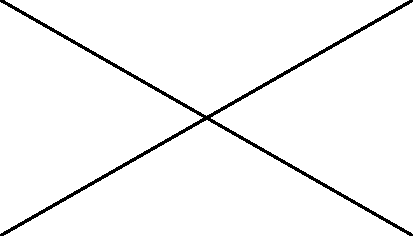
\includegraphics[width=\ScaleIfNeeded]{../image-missing}
	\\\texttt{ [NodeGraph]<>--[NodeMatch]<>--[Node]}
	\\\texttt{~~~~~~~~~~~1~~~1…n~~~~~~~0…n~~~2~~~~~}
	\caption{...}
	\label{fig:impl-node-match-model}
}

Da die \textproc{Analyse} für jedes Segment immer jeweils links- und rechtsseitig nach Parallelen sucht, werden beim \textproc{NodesZuordnen} viele Zuordnungen doppelt gefunden, nämlich einmal in jeder Richtung.
Erneut vereinfachen die Eigenschaften der mathematischen Menge, hier der Menge aller Zuordnungen $C$, die Beschreibung des Algorithmus in Abschnitt~\ref{ch:node-match-algorithm}.
Weil \code{NodeMatch}-Objekte wie beschrieben die Mengeneigenschaften implementieren, können sie leicht direkt im Java Collections Framework verwendet werden, hier als \code{Set<NodeMatch>} (Menge von \code{NodeMatch}-Objekten).
Da der Datentyp \code{NodeMatch} gleichzeitig die Schnittstelle \code{Set<Node>} implementiert, hat die Menge aller Zuordnungen implizit den Typ \code{Set<Set<Node>>}, ist also eine Menge \emph{von Mengen} von \term{nodes}, was genau der formalen Anforderung in Abschnitt~\ref{ch:node-match-algorithm} entspricht.

% TODO: SourceNode, nicht Node. Spielt das eine Rolle, oder versteht man es auch so?

Punktezuordnungen und Segmente ergeben gemeinsamen einen gemischten Graphen des zu generalisierenden Netzes.
Als parallel erkannte Segmente sind über deren \term{nodes} derart einander zugeordnet, dass sich eine gemeinsame Mittellinie als Verknüpfung der Mittelpunkte derjenigen Kanten im Graphen, welche die Punktezuordnungen darstellen, leicht finden lässt.
Zur Definition des Graphen genügt die Menge aller Punktezuordnungen, wenn über die einzelnen Punkte die mit ihnen verknüpften Segmente ermittelbar sind.

% TODO: ist hier der Fall, über addSegment(), welches in AbstractLine passiert. Sollte vielleicht weiter oben in 4.3.1 erwähnt werden.



\subsection{Liniengeneralisierung}

Für 4.3.3 ergibt sich folgendes Datenmodell/Klassenstruktur:
\onefigure{ht}{
% [GeneralisedLines]1 <>-- 0…n[ResultLine (Section/GeneralisedSection)]0…n <>-- 2…n[Node]
	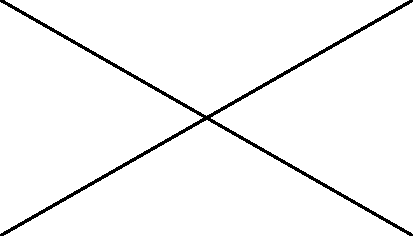
\includegraphics[width=\ScaleIfNeeded]{../image-missing}
	\\\texttt{ [GeneralisedLines]<>--[ResultLine]<>--[Node]}
	\\\texttt{~~~~~~~~~~~~~~~~~~1~~~0…n~~~~~~~~0…n~~2…n~~~~}
	\caption{...}
	\label{fig:impl-generalisation-model}
}

% TODO: 4.3.4 spricht hier von Segmenten, die aneinandergehangen werden. Eventuell passiert das hier mit Nodes? Nochmal prüfen! Macht aber eigentlich keinen großen Unterschied.
% ...

\begin{itemize}
\item im Wesentlichen: welche Pointer werden an Segmente drangehangen und wie hängen ResultLine, *Section und GenLines zusammen?
\end{itemize}



\subsection{Zusammenfassung und ggf. Datenfluss/Interaktionswege}

\begin{itemize}
\item Integration der beschriebenen Klassen zu einem funktionierenden System
\item \code{Combiner} = Façade
\item ggf. Datenfluss/Interaktionswege
% (weichen im imperativen Code teils deutlich von funktional formulierten Algorithmen ab)
\end{itemize}

% TODO: Big Renaming #4 (optional)
%1: de.thaw.thesis.comb -> de.thaw.comb
%2: Dataset
% special uses (to be reconsidered):
% - Output for debugging
% - Corr.Graph to get all segments
% - Gen.Lines to get all segments and to get midPoints
% - AbstractSegment for debugging (parallelFragment sink etc.)
%3: code currently contains a lot of special-cases for debugging as well as testing:
% - CombinerMain: iterations / combineLines2
% - MyAnalyser: evaluateTags
% - pervasive debug output needs to be overhauled; perhaps as a common sink/listener



% ===========================
% Anhänge:
% - komplettes ER-Modell
% - komplette Klassenstruktur
% - Auflösung der verwendeten Bezeichner in Kap. 4 vs. im Source:
% SEGMENTIERUNG: OsmWay.segmentation
% SPLITTEN: SplitQueueIterator=S' (in Combiner.splitSegments), AbstractLine.splitCloseParallels()=für alle n/t, T enthält schon eine Parallitätsprüfung (warum? - in splitTargets/closeParallels)
% NAHESEGMENTE: Combiner.regionaliseSegments (arbeitet auf SourceSegments, also auf S statt S' und wurzel(s) statt s, weil so die Schnittmengenprüfung nicht wiederholt ausgeführt werden muss und damit ein Spatial Index erleichtert/ermöglicht wird)
% HÜLLE: SourceSegment.envelope
% FUSSPUNKT: AbstractSegment.findPerpendicularFoot
% ANALYSE: AbstractSegment.analyse
% PARALLEL: SourceSegment.closeParallels / MyAnalyser
% DISTANZ: MyAnalyser.evaluate
% NODESZUORDNEN: NodeGraph.createGraph
% ZUSAMMENFASSEN: ... (GeneralisedLines/GeneralisedSection)



\section{Schwierigkeiten bei der Umsetzung}
\label{ch:impl-difficulties}

% TODO: "Während der Entwicklung wurde versucht, so viel existierenden Code in Form von \term{frameworks} wiederzuverwenden wie möglich. Diese Bestrebung verursachte Probleme, wie auch später in Abschnitt~\ref{ch:impl-difficulties} geschildert wird."

% TODO: commit log, Notizen und alte Screenshots/Testdaten aufarbeiten
% hier NICHT Probleme mit dem Generalisierungsergebnis oder der Korrektheit der Algorithmen besprechen (gehört zu 6)



\subsection{Eigenschaften der Sprache}

\begin{itemize}

\item
Dass in den zur Verfügung stehenden Java-\term{frameworks} nicht bereits geeignete Datenstrukturen für die Arbeit mit Segmenten existieren, hat einiges an zusätzlicher Arbeit verursacht.
Das Aufbauen der Datenstrukturen war lehrreich, aber zeitaufwändiger als erwartet.

\item
Die Entwicklung von der Idee für einen Algorithmus hin zu einer für komplexe Geodaten praxistauglichen Implementierung kann als iterativer Prozess verstanden werden.
Unter dem Eindruck der Ergebnisse früher Versionen können Algorithmus und Implementierung nach und nach verfeinert werden.
% http://de.wikipedia.org/wiki/Prototyping_(Softwareentwicklung)#Evolution.C3.A4res_Prototyping
Die Wahl von Java als streng typisierte Sprache erschwerte jedoch dieses Vorgehen.
%Der Zeitaufwand dafür, elegante Klassenstrukturen aufzubauen, wurde vom Verfasser unterschätzt.

Die strenge Typisierung hat die Implementierung aufwändiger gemacht und den Fokus (bei vorgegebenem Zeitrahmen für die Arbeit) somit notwendigerweise ein Stück weit verschoben weg von Algorithmusentwicklung und -beurteilung hin zu den Details objektorientierter Programmierung.
Dies war so vor Beginn nicht absehbar.
% denn nur ich+Jochen waren Programmierer, aber nur die offiziellen Betreuer haben akad. Erfahrung
Möglicherweise wäre eine dynamisch typisierte Skriptsprache wie Perl für das explorative Vorgehen geeigneter gewesen.
% warum? -> erfordert Anpassungen der Strukturen von Algorithmen und Daten

\item
Erwartungsgemäß war das Java Collections Framework eine große Hilfe.

\item
Die Idee, nicht nur im Algorithmus, sondern auch in der Typenhierarchie Segmente als Vektoren zu behandeln, stellte sich als sehr hilfreich heraus.
Es ist denkbar, dass eine Sprache mit Operatorüberladung wie Perl diesen Vorteil noch besser hätte ausnutzen können.

\end{itemize}



\subsection{Ein- und ausgabe von Geodaten}

\begin{itemize}

\item
Zwar ist diese Arbeit ausdrücklich aus \osm\ fokussiert, beim Prototyping stellte sich allerdings heraus, dass das direkten Einlesen von \osm-Daten etwas schwieriger war als erwartet.
Die Eingabe wurde daher zunächst über die Shapefiles der Geofabrik realisiert.
Auch die Ausgabe erfolgt zunächst als Shapefile, damit das Generalisierungsergbnis leicht mit gängiger Software betrachtet werden kann.
Schnittstellen für Ein- und Ausgabe von \osm-Daten zu ergänzen, sollte aber nicht allzu schwierig sein.

\item
Die Shapefiles der Geofabrik enthalten aus technischen Gründen veränderte Attribute, nicht die Original-\osm-\term{tags}.
Diesem Problem wurde begegnet, indem ein Adapter die aus den Shapefiles gelesenen Attribute wieder zurück in das \osm-Format wandelt, ohne dass dies für den Combiner sichtbar wird.
% Adapter pattern: io.ShapeTagsAdapter

\item
Die Nutzung des \term{frameworks} GeoTools zur Ein- und Ausgabe von Geodaten war problematisch.
Zwar bietet GeoTools umfangreiche Unterstützung für verschiedene Datenformate, jedoch sind diese I/O-Klassen von GeoTools eher umständlich zu benutzen, ihr Interface ist nicht stabil und sie sind sehr teuer.
Eine Lösung hierfür zu entwickeln, war sehr zeitaufwändig.

Um die Datenausgabe auf eine akzeptable Geschwindigkeit zu beschleunigen, werden diese nun im GeoJSON-Format ausgegeben (implementiert als reine Textausgabe, was sehr billig ist).
Das GeoJSON wird anschließend mit GDAL in ein Shapefile konvertiert.
Insgesamt ist diese Lösung um ein Vielfaches schneller als der Shapefile-Support von GeoTools.

(Allerdings wurde der Shapefile-Support in Geotools neu implementiert; ob dies die Probleme löst, wurde noch nicht getestet.)
% http://web.archive.org/web/20130926213903/http://docs.codehaus.org/display/GEOTOOLS/Migrate+shapefile+to+shapefile-ng

\item
Außer dem eigentlichen Generalisierungsergebnis kann die entwickelte Software auch zahlreiche zusätzliche Geodatensätze ausgeben, die das Verständnis von der Arbeitsweise des Algorithmus bei Anwendung auf Real-World-Daten verbessern und auch beim Debuggen hilfreich sind.
Diese Ausgaben sind in keiner Weise optimiert.

\end{itemize}



\subsection{Sonstiges: Flexibilität und Effizienz}

\begin{itemize}

\item
Die Definition des Spezialfalls, auf den die Arbeit beschränkt werden soll, in einem eigenen Paket \code{highway} vom Rest des Combiners zu trennen und sie damit leicht austauschbar zu machen, war grundsätzlich eine gute Idee.
Diese Trennung ist allerdings bisher nur begonnen worden und konnte aus Zeitgründen nicht bis zum Abschluss der Arbeit beendet werden; angesichts der ausdrücklichen Beschränkung in der Aufgabenstellung auf nur den ausgewählten Spezialfall war das aber auch streng genommen gar nicht notwendig.
% betrifft insb. die Klassen Line, AbstractLine, io.InputDataset, io.ShapeReader sowie GeneralisedSection/Section
% "In der vorliegenden Software akzeptieren die Segmente den Besuch eines Objekts, das die Schnittstelle \code{Analyser} implementiert. Dieses Objekt enthält die Implementierungen der Algorithmen \textproc{Parallel} und \textproc{Distanz}." --- stimmt das überhaupt schon?

\item
Im Unterschied zur formalen Definition in Abschnitt~\ref{ch:analyse-algorithm} sind $parallelLinks$ und $parallelRechts$ nicht als homogene binäre Relation auf Segmenten implementiert, sondern als Relation zwischen Segmenten und \emph{Mengen} von Segmenten.
Mit anderen Worten: Es wird nicht jeweils nur ein einziges Segment je Seite als „parallel“ markiert, sondern mehrere.
% es wird in der Tat wie theoretisch überlegt durch die reziproke Zuordnung sichergestellt, dass auch ohne Liste für jedes Paar eine Zuordnung erstellt wird
Auf die Korrektheit der Algorithmen hat dies keinen Einfluss.
Zwar entstehen beim \textproc{NodesZuordnen} zunächst mehr Zuordnungen.
Dies sind jedoch Duplikate, die aufgrund der Mengeneigenschaft entfallen (vergleiche Abschnitt~\ref{ch:impl-node-match}).
Es stellt sich hier also die Frage, welche Implementierungsvariante mit dem Java Collections Framework am effizientesten umzusetzen ist.
Ein \term{profiling} wurde noch nicht durchgeführt.
% => Optimierungspotenzial

\item
Zahllose geschachtelte Schleifen lassen Schlimmes für die Effizienz befürchten, jedoch wird in vielen Fällen nur über eine Menge der Mächtigkeit $2$ iteriert
% (teils weniger, wie die Untersuchung zu realParallels ergab)
und in anderen Fällen wird durch \textproc{NaheSegmente} die Größe der Menge stark begrenzt; deshalb ist der Rechenaufwand in der Praxis gar nicht mal so schrecklich hoch.
Der Speicheraufwand und insbesondere das Verhalten des \term{garbage collectors} ist ein größeres Problem; hier besteht Optimierungspotenzial.

\end{itemize}



% single-chapter commands
\onlyinsubfile{\listoffigures}
%\onlyinsubfile{\listoftables}
\onlyinsubfile{% global bibliography settings

\nocite{*}  % include works in bibliography that aren't cited anywhere in the document (for debugging)

\setbibpreamble{Die Literaturangaben sind alphabetisch nach den Nachnamen der Autoren sortiert. Bei mehreren Autoren wird nach dem ersten Autor sortiert.\par\bigskip\bigskip}

\bibliography{../references-papers,../references-manual}
%\bibliography{../references-manual}
}
\end{document}
